\title[DS - Introduction]{\textbf{Distributed Algorithms}\\Introduction}

\begin{document}

\begin{frame}
\titlepage
\end{frame}

\section{Getting Started}

\subsection{Two generals}

\begin{frame}{Two generals}
A thought experiment~\cite{two-generals}:	
\begin{center}
\begin{figure} 
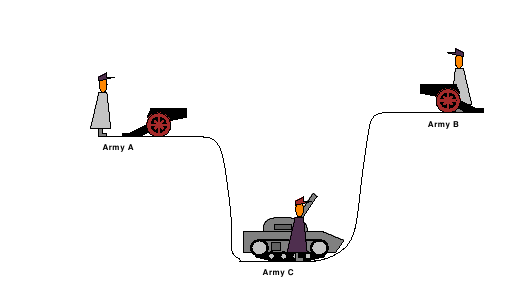
\includegraphics[width=0.8\textwidth]{figs/01/two-generals.png}
\end{figure}
\end{center}

\end{frame}
	
\begin{frame}{A potential solution}
	
\BI
\item General $A$: attack at dawn!
\pause
\item General $B$: ack, attack at dawn!
\pause
\item General $A$: ack ack, attack at dawn!
\pause
\item General $B$: ack ack ack, attack at dawn!
\item \ldots
\EI

\pause
\begin{theorem}
Under this scenario, there is no solution for the Two Generals Problem
\end{theorem}
\pause
\begin{proof}
By contradiction on the number of messages exchanged.
\end{proof}

\note{

\BI
\item Let's assume (by contradiction) that there is at least one solution to this
problem under this scenario. 
\item If there is one, there could be many. 
\item If there
are many, we can find one which uses the minimum number of messages. 
\item Take
the last message of this protocol: it can be received or it can be lost
\item
The protocol should work in both cases. So we could avoid sending it
at all! 
\item The resulting protocol uses less messages than the minimum, which is a contradiction
\EI
}


\end{frame}

\begin{frame}{Reality Check}	
	
\begin{block}{Atomic Commit}
An atomic commit is an operation in which a set of distinct changes is applied 
as a single operation.
\end{block}

\bigskip
Example: ATM's withdrawal
\BI
\item You whitdraw $100$ euro from an ATM in Trento
\item Your balance should be decreased by $100$ euro
\EI

\end{frame}

\begin{frame}{A pragmatic solution}

%% TODO: Look at the binomial distribution, as suggested by Vimal.
	
	
\begin{block}{Probabilistic protocol}
\BI
\item Assuming messengers are caught independently of each other with probability $p$
\BI
\item General $A$:
\BI
  \item Send $n$ messengers
  \item Attacks no matter what
\EI
\item General $B$:
\BI
  \item Attacks if receives at least one messenger 
\EI
\EI
\item $p^n$ is the probability that the attack will be uncoordinated
\EI
\end{block}

\bigskip
Trade-off:
\BI
\item We can decrease the \emph{probability} of failure by increasing $n$...
\item But at the additional cost of sending more messengers!
\item Without be ever certain that the attack will be coordinated!
\EI
\end{frame}

\subsection{Common Knowledge}

\begin{frame}{Muddy children}
\BI
\item $n$ children go playing 
\item Children are truthful, perceptive, intelligent
\item Mom says: “Don’t get muddy!”
\item A bunch (say, $k$) get mud on their forehead
\item Daddy comes, looks around, and says “Some of you got a muddy forehead”
\item Daddy repeatedly ask: “Do you know whether you have a muddy forehead?”
\EI

\bigskip
What happens?

\bigskip
{\footnotesize Slides from Lorenzo Alvisi}
\end{frame}


\begin{frame}{Muddy children}
\begin{theorem}
\BI
\item The first $k-1$ times Daddy asks, they children says “No”
\item The $k$-th time, the $k$ children say “Yes”.
\EI
\end{theorem}

\begin{proof}
By induction on $k$
\end{proof}

\note{
\BI
\item  Let $k=1$.
\BI
\item The first time daddy asks, the child with mud on his forehead say
  yes. 
\item Because all the other have no mud, and someone has mud on his
  forehead, it must be him.
\EI
\item Let $k>1$. 
\BI
\item Every child with mud see $k-1$ children with mud on
  the forehead. 
\item If there were $k-1$ children with mud, they would have
  said yes at the $(k-1)$-th time daddy asks, but they didn't. 
\item So there are
  actually $k$ children with mud, and they all say yes at the $k$-th
  time daddy asks.
\EI
\EI
}

\end{frame}

\begin{frame}{Muddy children}
\begin{block}{Variation 1}
\BI
\item Suppose $k>1$
\item Every one knows that someone has a dirty forehead before Dad announces it
\item Does Dad still need to speak up?
\EI
\end{block}

\pause
\BI
\item Let $p$ = “Someone’s forehead is dirty” 
\item Every one knows $p$
\item But, unless the father speak, if $k = 2$ not every one knows that everyone knows $p$!
\item Suppose $A$ and $B$ are dirty. Before the father speaks $A$ does not know whether $B$ knows $p$
\item If $k = 3$ , not every one knows that every one knows that every one knows $p$ ...
\EI


\end{frame}

\begin{frame}{Muddy children}
\begin{block}{Variation 2}
... the father took every child aside and told them individually (without others noticing) that someone’s forehead is muddy?
\end{block}
\begin{block}{Variation 3}
... every child had (unknown to the other children) put a miniature microphone on every other child so they can hear what the father says in private to them?
\end{block}
\end{frame}

\begin{frame}{Two generals, reloaded}
\BI
\item There is an entire logic that formalizes what knowledge participants acquire while running a protocol
\item J. Halpern and Y. Moses. \emph{Knowledge and Common Knowledge in a Distributed Environment}. E.W. Dijkstra Prize 2009.
\item Solving the Two Generals Problem requires common \emph{knowledge}
\BI
\item  “everyone knows that everyone knows that everyone knows...” 
\EI
\EI
\bigskip
But:
\BI
\item Common knowledge cannot be achieved by communicating through unreliable channels
\EI


\end{frame}

\begin{frame}{A common knowledge puzzle}

\textbf{Albert} and \textbf{Bernard} just become friends with \textbf{Cheryl}, and they want to know when her birthday is. \textbf{Cheryl} gives them a list of 10 dates:

\BI
\item May 15,16,19
\item June 17,18
\item July 14,16
\item August 14,15,17
\EI

\textbf{Cheryl} then tells \textbf{Albert} and \textbf{Bernard} separately the month and the day of her birthday respectively.

\BI
\item \textbf{Albert}: I don't know when \textbf{Cheryl}'s birthday is, but I know that \textbf{Bernard} does not know too.
\item \textbf{Bernard}: At first I didn't know when \textbf{Cheryl}'s birthday is, but I know now.
\item \textbf{Albert}: Then I also know when \textbf{Cheryl}'s birthday is
\EI
	
\end{frame}



\subsection{Byzantine generals}

\begin{frame}{Byzantine generals}
\begin{block}{Scenario~\cite{pearls-of-theory}}
\BI
\item $n$ Byzantine generals encircling a city
\item They must decide whether to attack or retreat!
\item Messengers are \emph{reliable} and \emph{synchronous}
\item Generals may be traitors
\item Nobody knows which generals are traitors
\EI	
\end{block}

\begin{block}{Problem specification}
The generals require an algorithm to reach an agreement such that (i) all loyal generals decide on the same plan of action and (ii) a small number of traitorous generals cannot cause the loyal generals to adopt different plans.
\end{block}

\end{frame}

\begin{frame}{A potential solution}

\BI
\item Wait for a majority of generals to agree
\EI

\pause
\bigskip
WRONG! Possible scenario:
\BI
\item $3$ generals
\item $1$ vote “attack”, $1$ vote “retreat”
\item $1$ traitorous general:
\BI
\item sends a vote “attack” to the “attack” general
\item sends a vote “retreat” to the “retreat” general
\EI
\EI

\end{frame}

\begin{frame}{The problem is solvable}

\begin{block}{Byzantine Fault Tolerance (1982)}
\BI
\item L. Lamport, R. Shostak, M. Pease, \emph{The Byzantine Generals Problem}, ACM Trans. on Programming Languages and Systems, 4(3):382--401, 1982. 
\item A protocol that given $n$ processes,can tolerate up to $t$ traitorous generals with $n \geq 3t+1$
\item Example: $4$ generals can tolerate up to 1 “byzantine” general
\EI
\end{block}

\begin{block}{Practical Byzantine Fault Tolerance (2002)}
\BI
\item M. Castro and B. Liskov, \emph{Practical Byzantine Fault Tolerance and Proactive Recovery}, ACM Trans. on Computer Systems, 20(4):398--461, 2002.
\item PBFT triggered a renaissance in BFT replication research
\item Still going on...
\EI
\end{block}
\end{frame}

\begin{frame}{Reality Check}
\BI
\item BFT sponsors in 1982
\BI
  \item NASA
  \item The Ballistic Missile Defense System Command
  \item Army Research Office
\EI
\bigskip
\item Nancy Lynch's book on Distributed Systems:\\
\BI
\item
\emph{The agreement problem is a simplified version of a problem that originally
arose in the development of on-board aircraft control systems.
}
\EI
\bigskip
\item BitCoin, a peer-to-peer digital currency system, is based on BFT.
\bigskip
\item The 8-hour downtime of Amazon S3 in July 2008 is a well-known example
  of what happens when you don't use BFT.
\EI
\end{frame}

\subsection{Summary}


\begin{frame}{Take-home lessons}
\BI
\item We need to properly \emph{model} our distributed systems
\BI
\item Reliable / unreliable communication
\item Benign / malicious processes
\EI
\bigskip
\item Solutions depend on the underlying model
\BI
\item “Approximate” or “probabilistic” solutions
\item “Bounded” solution
\item No solution at all!
\EI
\bigskip
\item Coordinating multiple processes is difficult
\BI 
\item Unexpected events: failures, malicious behavior
\item Lack of common knowledge
\EI
\EI
\end{frame}

\section{Themes of the course}

\subsection{Impossible vs practical}

\begin{frame}{Theory vs practice}
\begin{block}{Yogi Berra says:}
In theory, theory and practice are the same. \\
In practice, they are not.
\end{block}

\pause
\begin{block}{Yogi Berra}
\begin{minipage}{0.20\textwidth}

\includegraphics[width=\textwidth]{figs/01/yogi.jpg}
\end{minipage}
\begin{minipage}{0.75\textwidth}
\BI
\item “Always go to other people's funerals, otherwise they won't go to yours”
\item “I really didn't say everything I said”
\item “Nobody goes there anymore; it's too crowded”
\EI
\end{minipage}
\end{block}	

\end{frame}

\begin{frame}{First theme of the course}

\begin{block}{Impossible vs practical}
Several papers about \emph{impossibility results}:
{\footnotesize
\BI
\item M. Fischer, N. Lynch, M. Paterson. \emph{Impossibility of Distributed Consensus with One Faulty Process}. Journal of ACM, 32(2):374--382, 1985.
\item S. Gilbert, N. Lynch. Brewer's Conjecture and the Feasibility of Consistent, Available, Partition-Tolerant Web Services. ACM SIGACT News, 33(2):51-59, 2002.
\EI
}

\bigskip
Yet, many of these problems have \emph{practical solutions}:
{\footnotesize
\BI
\item T. Chandra and S. Toueg. \emph{Unreliable failure detectors for reliable distributed systems}. Journal of the ACM, 43(2):225--267, 1996.
\item L. Lamport. \emph{Paxos made simple}. ACM SIGACT News, 32(4):18--25, 2001.
\EI
}
\end{block}

\bigskip
A general tension in Computer Science:
\BI
\item {\footnotesize M. Vardi. \emph{Solving the Unsolvable}. Comm. of the ACM, 54(7):5, 2011}. 
\EI

\end{frame}

\subsection{Classical vs extreme distributed systems}

\begin{frame}{Beyond technology}
\begin{block}{The Spanish Flu, 1918-1920}
\BI
\item Pandemic: killed 20M people in a relatively short time, more than World War I
\item Virus goal: spread itself as quickly as possible
\item Unreliable environment:
\BI
\item viruses may be killed
\item transmission may fail
\EI
\item Transmission network is a complex graph
\EI
\end{block}

\end{frame}

\begin{frame}{Beyond technology}

\begin{block}{Flocks of birds}
\BI
\item Flying in a flock is good: 
	\BI
	\item probability of being killed by a predator is reduced
	\EI
\item Flying in a flock is bad: 
	\BI
	\item probability of finding (enough) food is reduced
	\EI
\item Birds self-organize themselves in a flock
\item No central authority
\EI
\end{block}

\end{frame}



\begin{frame}{Second theme of the course}

\begin{block}{Classical vs extreme distributed systems}
\BI
\item Classical distributed system problems include agreement, total order
  broadcast, atomic commit, replication, etc.
\item Extreme distributed system problems include self-* properties, 
  scalability, full decentralization, etc.
\EI
\end{block}

\begin{block}{Special issue on Springer Computing (Sept. 2012)}
Alberto Montresor, Gusz Eiben, Maarten van Steen, editors\\

\textit{“Modern distributed systems may nowadays consist of hundreds of
thousands of computers, ranging from high-end powerful machines to low-end
resource-constrained wireless devices. We label them as extreme distributed
systems, as they push scalability and complexity well beyond traditional
scenarios.”}

\end{block}

\end{frame}

\subsection{Syllabus}

\begin{frame}[shrink]{Topics}

\begin{columns}
\begin{column}{0.44\textwidth}
\BI
\item Introduction
\item Models
\item Time, clocks, events
\item Reliable broadcast
\item Epidemic protocols
\item Impossibility of consensus
\item Consensus and failure detectors
\item Complex networks
\item Replication
\item P2P
\EI
\end{column}
\begin{column}{0.56\textwidth}
\BI
\item Epidemics: Beyond dissemination
\item Atomic Commitment
\item Rollback and Recovery
\item Group Communication
\item Paxos
\item Practical Byzantine Fault Tolerance
\item Blockchains
\item Byzantine, altruistic, rational model
\item Distributed frameworks
\EI
\end{column}
\end{columns}

\end{frame}


\addtocontents{toc}{\newpage}

\section{Distributed Systems}

\subsection{Informal definition}

\begin{frame}{What is a distributed system?}
	
\begin{block}{Definition (pragmatic)}
A collection of independent, autonomous hosts connected through a
communication network. Host communicate via message passing to achieve some
form of cooperation.
\end{block}

\pause
\bigskip
\begin{block}{Definition (by negation)}
A parallel system where there are no:
\BI
\item shared, global clock
\item shared memory
\item accurate failure detection
\EI
\end{block}

\end{frame}

\begin{frame}{What is a distributed system?}

\begin{block}{Definition (optimistic)}
\begin{minipage}{0.15\textwidth}
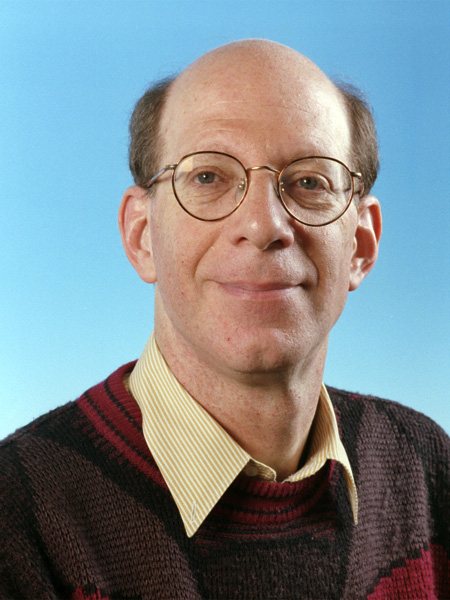
\includegraphics[width=\textwidth]{figs/01/tanenbaum.jpg}
\end{minipage}
\hfill
\begin{minipage}{0.80\textwidth}
A collection of independent computers that appears to its users as a single coherent system [Andrew Tanenbaum]
\end{minipage}
\end{block}

\pause
\smallskip
\begin{block}{Definition (pessimistic)}
\begin{minipage}{0.15\textwidth}
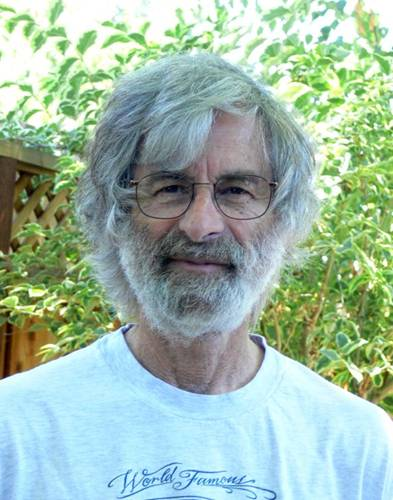
\includegraphics[width=\textwidth]{figs/01/leslie.jpg}
\end{minipage}
\hfill
\begin{minipage}{0.80\textwidth}
A distributed system is one in which the failure of a computer you did not even know existed can render your own computer unusable [Leslie Lamport]
\end{minipage}
\end{block}

\end{frame}

\begin{frame}{Motivation}
\begin{block}{Inherent distribution}
Applications which require sharing of resources or dissemination of information among geographically
distant entities are “natural” distributed systems
\end{block}

\bigskip
Examples:
\BI
\item Bank with several branches
\item Distributed file systems, shared devices, etc.
\EI
\end{frame}

\begin{frame}{Motivation}
	
\begin{block}{Distribution as an artifact}
Distribution may be an artifact of an engineering solution to satisfy some specific requirements such as:
\BI
\item fault-tolerance
\item increased performance / cost ratio
\item minimum level of Quality of Service (QoS)
\EI
\end{block}

\bigskip
Examples:
\BI
\item Replicated servers
\EI
\end{frame}

\begin{frame}{Independent failures}

\begin{block}{From distributed systems to failures}
\BI
\item Dependencies between hosts augment the effect of failures
\item Distributed systems make the life of developers more difficult
\item Availability example:
\BI
\item $n$ dependent hosts, probability of failure $p$
\item Availability: $(1-p)^n$
\EI
\EI
\end{block}
\bigskip
\begin{block}{From failures to distributed systems}
\BI
\item Providing a replicated service via multiple independent processes enables fault tolerance
\item Distributed systems should simplify the life of users
\BI
\item $n$ independent hosts, probability of failure $p$
\item Availability: $1-p^n$
\EI
\EI
\end{block}
\end{frame}

\begin{frame}{Parallel systems}

\begin{block}{Definition}
Multiple processors that:
\BI
\item  \emph{share memory}\\
Communication based on shared memory and synchronization mechanisms
\item \emph{share time}\\
Access to a common clock
\item \emph{share fate}\\
No independent failures
\EI
\end{block}
\end{frame}

\begin{frame}{The true spirit of distributed systems}
	
\BI
\item \textbf{Parallel systems} exploit determinism to achieve efficiency
\bigskip
\item \textbf{Distributed systems} address uncertainty created by:
\BI
\item multiplicity of control flows
\item absence of shared memory and global time
\item presence of failures	
\EI
\EI
\end{frame}

\subsection{Challenges}

\begin{frame}{Challenges -- blah, blah}

\BI
\item Heterogeneity
\item Openness
\item Security
\item Failure handling
\item Transparency
\EI

\end{frame}

\begin{frame}{Heterogeneity}

Levels:
\BI
\item Network
\item Computing hardware
\item Operating systems
\item Programming languages
\item Multiple implementations
\EI

\begin{block}{Middleware}
\begin{minipage}{0.45\textwidth}
Software layer that abstracts from the above providing 
a uniform computational model
\end{minipage}
\hfill
\begin{minipage}{0.45\textwidth}
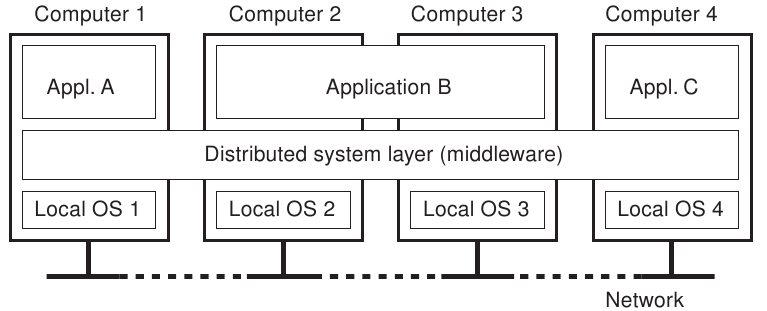
\includegraphics[width=\textwidth]{figs/01/middleware.png}
\end{minipage}

\end{block}


\end{frame}

\begin{frame}{Openness}
The degree to which a distributed system can be extended and re-implemented
\BI
\item Public interfaces
\item Standardization	
\EI

\bigskip
Examples:
\BI
\item Corba
\item Java2EE
\item .Net
\item Web Services
\EI
\end{frame}

\begin{frame}{Security aspects}

\BI
\item \textbf{Confidentiality}: avoiding the disclosure of the content of a message to a party distinct from the intended receiver
\bigskip
\item \textbf{Integrity}: avoiding the corruption of the transmitted contents by a third party
\bigskip
\item \textbf{Availability}: the capability of providing a service in spite of malicious behavior
\EI
\end{frame}

\begin{frame}{Failure handling}
\BI
\bigskip
\item Failure \textbf{detection} (e.g., message checksum)
\bigskip
\item Failure \textbf{masking} (e.g., email retransmission)
\bigskip
\item Failure \textbf{tolerance} (e.g., replicated servers)
\bigskip
\item Failure \textbf{recovery} (e.g., log files)
\EI

\bigskip
Distributed systems use a mix of these techniques
\end{frame}

\begin{frame}{Transparency}
\BI
\item \textbf{Access transparency}:  Hides differences in data representation and invocation mechanisms
\item \textbf{Location transparency}:  enables resources to be accessed without knowledge of their location
\item \textbf{Concurrency transparency}: enables several processes to operate concurrently using shared resources without interference 
\item \textbf{Replication transparency}: enables multiple resource instances to be used to increase reliability and performance without knowledge of the replicas by users
\item \textbf{Failure transparency}: enables the concealment of faults, allowing users and application programs to complete their tasks despite the failure of hardware or software components.
\item \textbf{Migration transparency}: allows the movement of resources and clients within a system without affecting operations
\EI
\end{frame}


\section{Conclusions}

\begin{frame}{What's next in the course?}
\BI
\item Distributed system modeling
\BI
\item Which kind of failures exist? 
\item Which kind of failures we tolerate?
\EI
\bigskip
\item Problem specification
\BI
\item Formal description of the problem
\EI
\item Algorithms, algorithms, algorithms
\BI
\item Pseudo-code descriptions of algorithms
\EI
\bigskip
\item Proofs
\BI
\item Just writing the code is not enough!
\item Sometimes, impossibility proofs
\EI
\bigskip
\item Reality checks
\BI
\item Learn about real systems where these protocols are applied
\EI
\EI
\end{frame}


\section{Bibliography}

\begin{frame}{Reading material}

{\footnotesize
\bibliographystyle{abbrv}
\bibliography{../references}  
}

\end{frame}


\begin{frame}{Reality Check: Interesting links}

\BI
\item \href{http://status.aws.amazon.com/s3-20080720.html}{\underline{The S3 incident}}
\item \href{http://cacm.acm.org/magazines/2011/7/109895-solving-the-unsolvable/fulltext}{\underline{Solving the unsolvable}}
\item \href{http://queue.acm.org/detail.cfm?id=1142044}{\underline{The rise and fall of Corba}}
\item \href{https://www.somethingsimilar.com/2013/01/14/notes-on-distributed-systems-for-young-bloods/}{\underline{Notes on Distributed Systems for Young Bloods}}
\EI

\end{frame}



\end{document} 

